 \documentclass[a4paper, 10pt, final]{article}

\usepackage{a4wide}

\usepackage{charter}
\usepackage{verbatim}
\usepackage{amsfonts}
\usepackage{amsmath}
\usepackage{amsthm}
\usepackage{amssymb}
%\usepackage[integrals]{wasysym}
%\usepackage{mathrsfs}
%\usepackage[mathcal]{euscript}
\usepackage{listings}
\usepackage{graphicx}
\usepackage{multirow}
\usepackage{multicol}
\usepackage{hyperref}
\usepackage{float}
\usepackage[small,bf]{caption}
\usepackage{synttree}
%\usepackage{pst-node}
%\usepackage{xypic}
\usepackage[table]{xcolor}
\usepackage{subfig}
%\usepackage{ulem} %use \normalem after begin document
\usepackage[authoryear]{natbib}

% Settings
\parindent=5pt
\parskip=8pt plus 2pt minus 4pt
\lstset{language=Matlab, basicstyle=\scriptsize,
    showstringspaces=false, numbers=left, stepnumber=1, numberstyle=\tiny, frame=tb}


\title{Statistical Methods for Machine Learning \\ Mandatory Project 2}
\author{Kasper Steenstrup\\Michael Andersen\\Esben Skaarup}
\date{\today}

\hypersetup{
colorlinks,%
citecolor=black,%
filecolor=black,%
linkcolor=black,%
urlcolor=black,%
bookmarksopen=false,
pdftitle={Statistical Methods for Machine Learning - Mandatory Project 2},
pdfauthor={Kasper Steenstrup, Michael Andersen \& Esben Skaarup}
}

\begin{document}
\maketitle

\subsection*{Question 2.1}

We calculate the RMS error for the to models, which is displayed in
table \ref{tab:q21} along with the min and max over 50
calculations. In the first model the RMS error is lower than the
other, the first model min and max is also closer. Based on this fact,
we see that the first model is better.

\begin{table}[!htbp]
  \centering
  \begin{tabular}{| l | l | l | l |}
    \hline
    {}		& RMS		& Max		& Min \\
    \hline
    Train1	& 4.4071	& 4.5634	& 4.2075 \\
    \hline
    Test1	& 4.5723	& 5.3269	& 3.9773 \\
    \hline
    Train2	& 4.8466	& 5.0046	& 4.5746 \\
    \hline
    Test2	& 4.9268	& 6.0025	& 4.2679 \\
    \hline
  \end{tabular}
  \label{tab:q21}
\end{table}


I figur \ref{fig:q2} the four RMS error for \alpha in the interval from
1 til 200 i displayet. As the figur indekeads the test data, have the
lowest error, and the firste model have the best results. The best value
for \alpha i one, sine the error get biggger the larger \alpha.

\begin{figure}[!htbp]
  \centering
  \includegraphics[width=0.6\textwidth]{./images/Q2.pdf}
  \caption{RMS for the 2 traning models and test models}
  \label{fig:q2}
\end{figure}



\subsection*{Question 2.6}

Setting the two equations equal as follows
\begin{align*}
p(x_1|\mathcal{C}_k)p(x_2|\mathcal{C}_k)p(\mathcal{C}_k) & = \frac{p(\mathcal{C}_k | x_1)p(\mathcal{C}_k | x_2)}{p(\mathcal{C}_k)} \iff \\
p(x_1|\mathcal{C}_k)p(x_2|\mathcal{C}_k)p(\mathcal{C}_k)p(\mathcal{C}_k) & = p(\mathcal{C}_k | x_1)p(\mathcal{C}_k | x_2) \iff
\end{align*}

Using Bayes theorem, we can rewrite
\[
p(\mathcal{C}_k | x_i) = \frac{p(x_i | \mathcal{C}_k)p(\mathcal{C}_k)}{p(x_i)}
\]
We do this for both factors on the right hand side and obtain

\begin{align*}
p(x_1|\mathcal{C}_k)p(x_2|\mathcal{C}_k)p(\mathcal{C}_k)p(\mathcal{C}_k) & = p(\mathcal{C}_k | x_1)p(\mathcal{C}_k | x_2) \iff \\
p(x_1|\mathcal{C}_k)p(x_2|\mathcal{C}_k)p(\mathcal{C}_k)p(\mathcal{C}_k) & = \frac{p(x_1|\mathcal{C}_k)p(\mathcal{C}_k)p(x_2|\mathcal{C}_k)p(\mathcal{C}_k)p(\mathcal{C}_k)}{p(x_1)p(x_2)} \iff \\
\frac{p(x_1|\mathcal{C}_k)p(x_2|\mathcal{C}_k)p(\mathcal{C}_k)p(\mathcal{C}_k)}{p(x_1|\mathcal{C}_k)p(\mathcal{C}_k)p(x_2|\mathcal{C}_k)p(\mathcal{C}_k)} & = p(x_1)p(x_2)
\end{align*}

We therefore see that the normalization constant is $p(x_1)p(x_2)$.

This can also be seen by applying Bayes theorem to $p(\mathcal{C}_k|x_1, x_2)$
\begin{equation*}
p(\mathcal{C}_k|x_1, x_2) = \frac{p(x_1|\mathcal{C}_k)p(x_2|\mathcal{C}_k)p(\mathcal{C}_k)}{p(x_1)p(x_2)}
\end{equation*}
From the above it can be seen that the normalization constant making
sure that the posterior distribution integrates to one is also
$p(x_1)p(x_2)$. As noted in the book the marginal distribution
$p(x_1,x_2)$ do typically not factorize under this model.

The result of running \emph{case26.m} looking at the shared covariance
the contours are simply mirrored in the decision boundary, which is
linear. The independent covariance becomes apperent as the contours of
the densities are formed according to the data the are based
on. Therefore the blue contours are streched more than the red
contours. The decision boundary resembles a hyperbola as in question
2.4.


% \subsection*{Question 2.7}

Figure \ref{fig:q27.1} shows the error as a function of $k$.  The
error seems to be lowest when $k = 7$. When $k < 7$ the decisions are
made from too few points, and over-fitting will occur.  Larger values
of $k$ will cause the model to be too simple.

\begin{figure}[!htbp]
  \centering
  \includegraphics[width=0.6\textwidth]{./images/q207_best_k.pdf}
  \caption{Test error for variating N with 200 training points.}
  \label{fig:q27.1}
\end{figure}

Figure \ref{fig:q27.2} shows the optimal values of $k$ for different
number of points $N$ in the training set.  Seemingly, as $N$ grows,
$k$ needs to be larger for the error to be minimized (apart from the
spike around $50-70$). This seems reasonable, as the additional
training points will cause the model to be more prone to over-fitting.
When more training points are used, but $k$ is raised correspondingly,
the level of detail, and therefore the error, in the model will remain
optimal.

\begin{figure}[!htbp]
  \centering
  \includegraphics[width=0.6\textwidth]{./images/q207_best_ks.pdf}
  \caption{Best k's (lowest test error) for variating N.}
  \label{fig:q27.2}
\end{figure}


\subsection*{Question 2.8}
\subsubsection*{1)}
Below in figure \ref{fig:q28decisiontree} can be seen the decision
tree for the situation.

% Sets the branch height.
%\branchheight{10em}
\begin{figure}[!htbp]
  \centering
  \synttree[\fbox{{}\quad{}} [No operation, $U(3)$\quad {}][\setlength{\unitlength}{0.5mm} \begin{picture}(1, 1) \put(-1,3){\circle{8}} \end{picture}[Live, $p=\frac{7}{10}$, $U(12)$][Die, $p = \frac{3}{10}$, $U(0)$]]]
  \caption{}
  \label{fig:q28decisiontree}
\end{figure}

\subsubsection*{2)}
The operation should be prefered if $U(3) < 0.7$, this is because in
order to obtain $U(12) = 1.0$, we need to have the operation. And as
there is $p(survive operation) = 0.7$, this results in $1.0 * 0.7 =
0.7$. Whereas the contrary $p(not survive operation) = 1 - p(survive
operation) = 1 - 0.7 = 0.3$, with $U(0) = 0.0$ we get $0.3 * 0.0 =
0.0$

\subsubsection*{3)}
We are to explain the calculations. It is simply a using Bayes theorem
to derive the posterior probability $p(\textrm{survive}|\textrm{pos})$
of the patient surviving given that the test was positive.

\subsubsection*{4)}
Yes, Dr. No should perform the operation, the chances of survival are
as given by the posterior probability in $3)$. Although there are
always a chance that it will fail and the patient will die.


\subsection*{Question 2.10}

% For making two columns of results
\begin{figure}[!htbp]
  \centering
  \subfloat[\label{subfig:q210Nh10}]{
  \begin{tabular}{|c|c|}
    \hline
    \multicolumn{2}{|c|}{Hidden units $= 10$} \\
    \hline
    Training error: 24.67\% & Test error: 29.38\% \\
    \hline
  \end{tabular}
  }
  \subfloat[\label{subfig:q210Nh30}]{
    \begin{tabular}{|c|c|}
      \hline
      \multicolumn{2}{|c|}{Hidden units $= 30$} \\
      \hline
      Training error: 25.33\% & Test error: 28.75\% \\
      \hline
    \end{tabular}
  } \\
  \subfloat[\label{subfig:q210Nh60}]{
    \begin{tabular}{|c|c|}
      \hline
      \multicolumn{2}{|c|}{Hidden units $= 60$} \\
      \hline
      Training error: 23.33\% & Test error: 28.00\% \\
      \hline
    \end{tabular}
  } 
  \subfloat[\label{subfig:q210Nh100}]{
    \begin{tabular}{|c|c|}
      \hline
      \multicolumn{2}{|c|}{Hidden units $= 100$} \\
      \hline
      Training error: 22.67\% & Test error: 28.31\% \\
      \hline
    \end{tabular}
  } \\
  \subfloat[\label{subfig:q210Nh130}]{
    \begin{tabular}{|c|c|}
      \hline
      \multicolumn{2}{|c|}{Hidden units $= 130$} \\
      \hline
      Training error: 22.67\% & Test error: 28.12\% \\
      \hline
    \end{tabular}
  } 
  \subfloat[\label{subfig:q210Nh200}]{
    \begin{tabular}{|c|c|}
      \hline
      \multicolumn{2}{|c|}{Hidden units $= 200$} \\
      \hline
      Training error: 23.33\% & Test error: 27.88\% \\
      \hline
    \end{tabular}
  } \\
  \subfloat[\label{subfig:q210Nh260}]{
    \begin{tabular}{|c|c|}
      \hline
      \multicolumn{2}{|c|}{Hidden units $= 260$} \\
      \hline
      Training error: 22.67\% & Test error: \textbf{27.31\%} \\
      \hline
    \end{tabular}
  } 
  \subfloat[\label{subfig:q210Nh300}]{
    \begin{tabular}{|c|c|}
      \hline
      \multicolumn{2}{|c|}{Hidden units $= 300$} \\
      \hline
      Training error: 24.00\% & Test error: 27.81\% \\
      \hline
    \end{tabular}
  } \\
  \subfloat[\label{subfig:q210Nh500}]{
    \begin{tabular}{|c|c|}
      \hline
      \multicolumn{2}{|c|}{Hidden units $= 500$} \\
      \hline
      Training error: 22.67\% & Test error: 29.31\% \\
      \hline
    \end{tabular}
  } 
  \subfloat[\label{subfig:q210Nh1000}]{
    \begin{tabular}{|c|c|}
      \hline
      \multicolumn{2}{|c|}{Hidden units $= 1000$} \\
      \hline
      Training error: \textbf{22.00\%} & Test error: 29.12\% \\
      \hline
    \end{tabular}
  }
  \caption{Show the result of running the neural network with various numbers of hidden units.}
  \label{fig:q210hidden}
\end{figure}


% First result

%


%






In figure \ref{fig:q1_1} can be seen the $100$ data points drawn from
the gaussian distribution with $\mu = [1.0~ 1.0]$ and $\Sigma = [0.3~
  0.2; 0.2~ 0.2]$. The correct $\mu$ is blue and $\widehat{\mu}$ is
marked with red.

\begin{figure}[!htpb]
  \centering
%  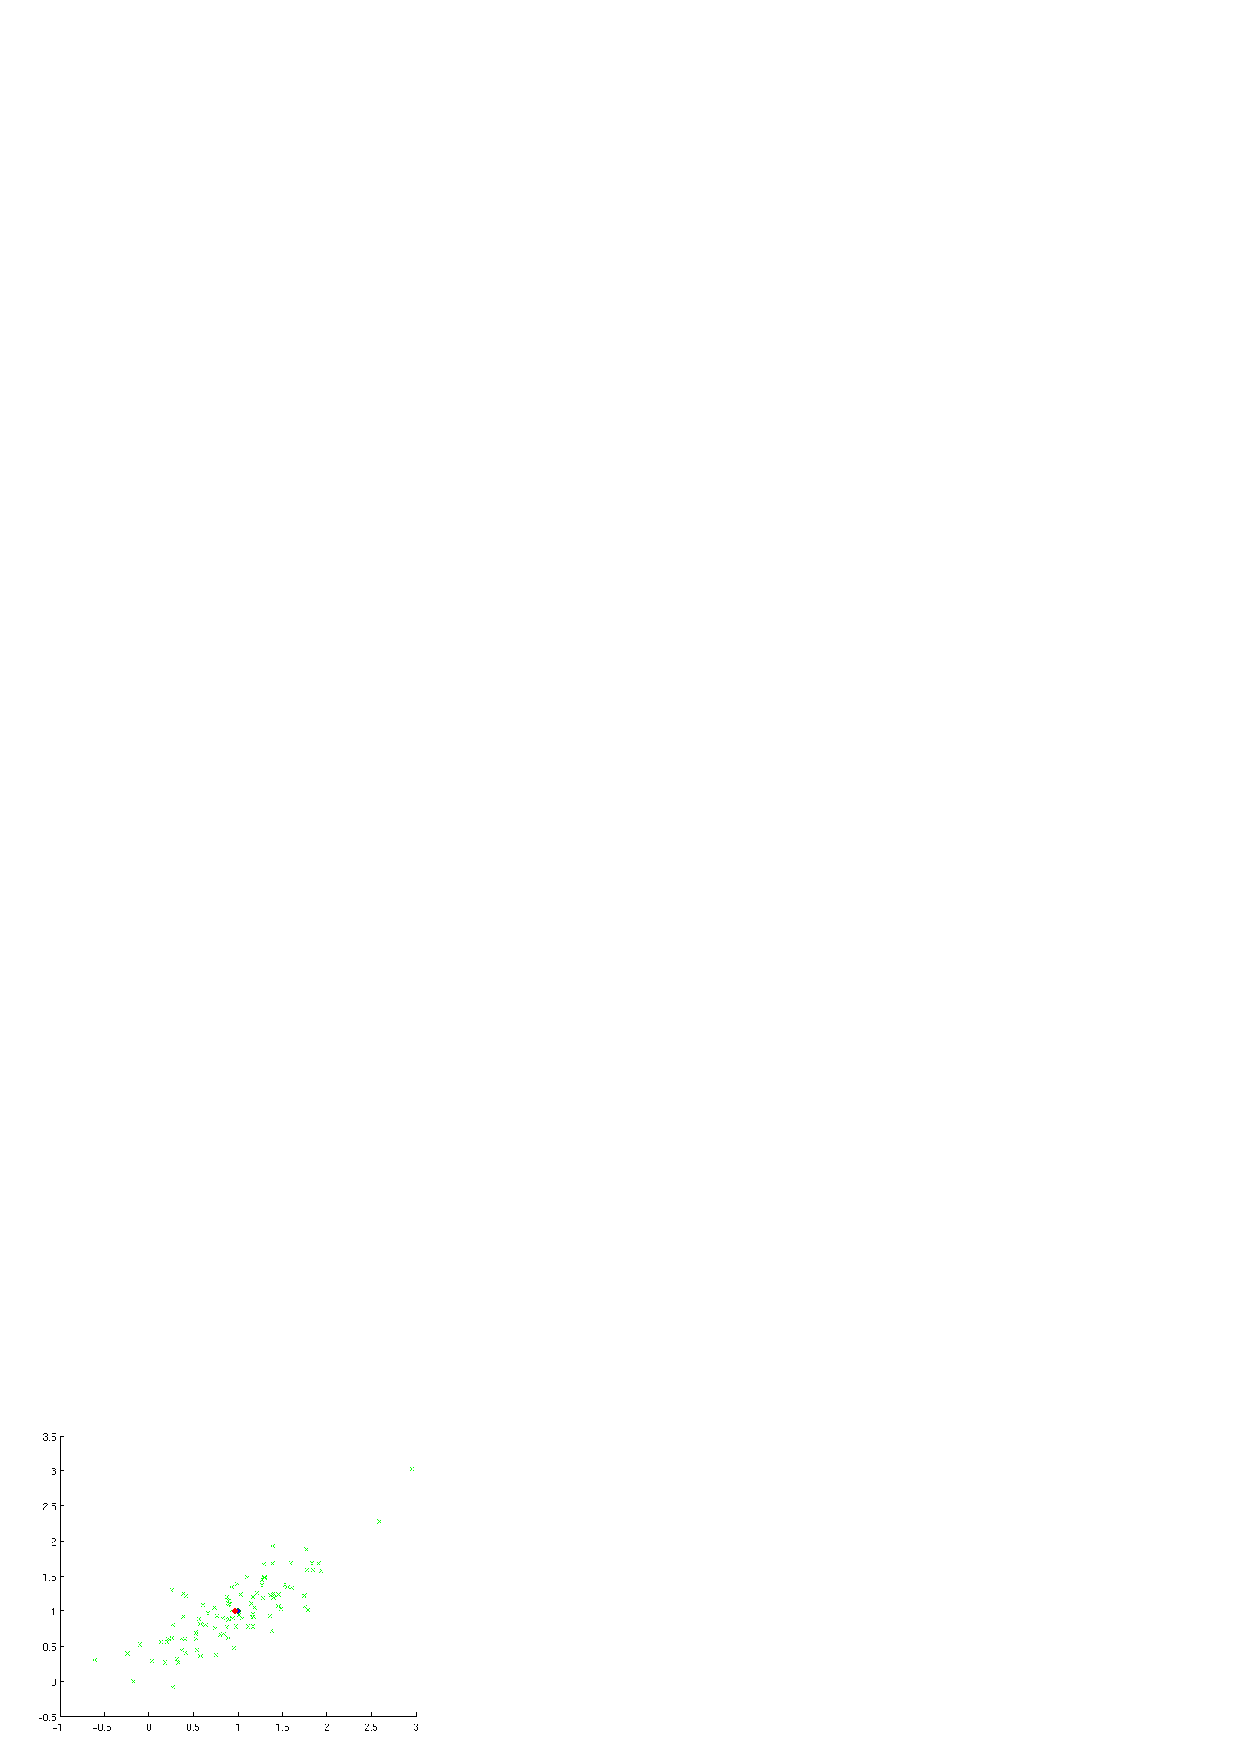
\includegraphics[width=0.6\textwidth]{images/q1_1}
  \caption{100 data points, correct mean with blue and estimated mean red.}
  \label{fig:q1_1}
\end{figure}

To quantify how much the estimated mean deviates from the correct
mean, we use usual euclidean distance between the two vectors.

Our distance is $0.0392$, which is not very much. This can also be
seen from the drawing, the points are placed really close.

The covariance matrix is also calculated on the training data:\\
$$\Sigma _{ML} = \left[
  \begin {array}{ccc}
    0.0082 & 0.0052 & 0.0067\\
    \noalign{\medskip}
    0.0052 & 0.0171 & 0.0199\\
    \noalign{\medskip}
    0.0067 & 0.0199 & 0.0241\\
  \end {array}
  \right]$$
% [0.0082~ 0.0052~ 0.0067; 0.0052~ 0.0171~ 0.0199; 0.0067~ 0.0199~ 0.0241]



%%%%%%%%%%%%%%%%%%%%%%%%%%%%%%%%%%%%%%%%%%%%%%%%%%%%%%%%%%%%%%%%%%%%
% Formal stuff

%\bibliographystyle{abbrvnat}
%\bibliography{bibliography}
%\addcontentsline{toc}{chapter}{Litteratur

\end{document}
